% Appendix Section

\section{Appendix}

\begin{frame}{Technical Implementation Details}
\textbf{Model Hyperparameters:}
\begin{table}[h]
\centering
\begin{tabular}{@{}ll@{}}
\toprule
\textbf{Parameter} & \textbf{Value} \\
\midrule
Learning Rate & 2e-5 \\
Batch Size & 16 \\
Max Sequence Length & 512 \\
Dropout Rate & 0.1 \\
Weight Decay & 0.01 \\
Warmup Steps & 500 \\
Training Epochs & 4 \\
\bottomrule
\end{tabular}
\end{table}

\vspace{0.5cm}
\textbf{Hardware \& Performance:}
\begin{itemize}
    \item Training time: 6 hours on NVIDIA V100
    \item Inference speed: 50ms per document
    \item Memory usage: 8GB GPU RAM during training
\end{itemize}
\end{frame}

\begin{frame}{Dataset Distribution Analysis}
\begin{columns}
\begin{column}{0.5	extwidth}
	extbf{Key Statistics:}
\begin{itemize}
    \item Total samples: 1,350
    \item Payment Terms: 20\%
    \item Termination: 18\%
    \item Confidentiality: 17\%
    \item Liability: 16\%
    \item Governing Law: 15\%
\end{itemize}
\end{column}
\begin{column}{0.5	extwidth}
\begin{center}
% Include dataset visualization
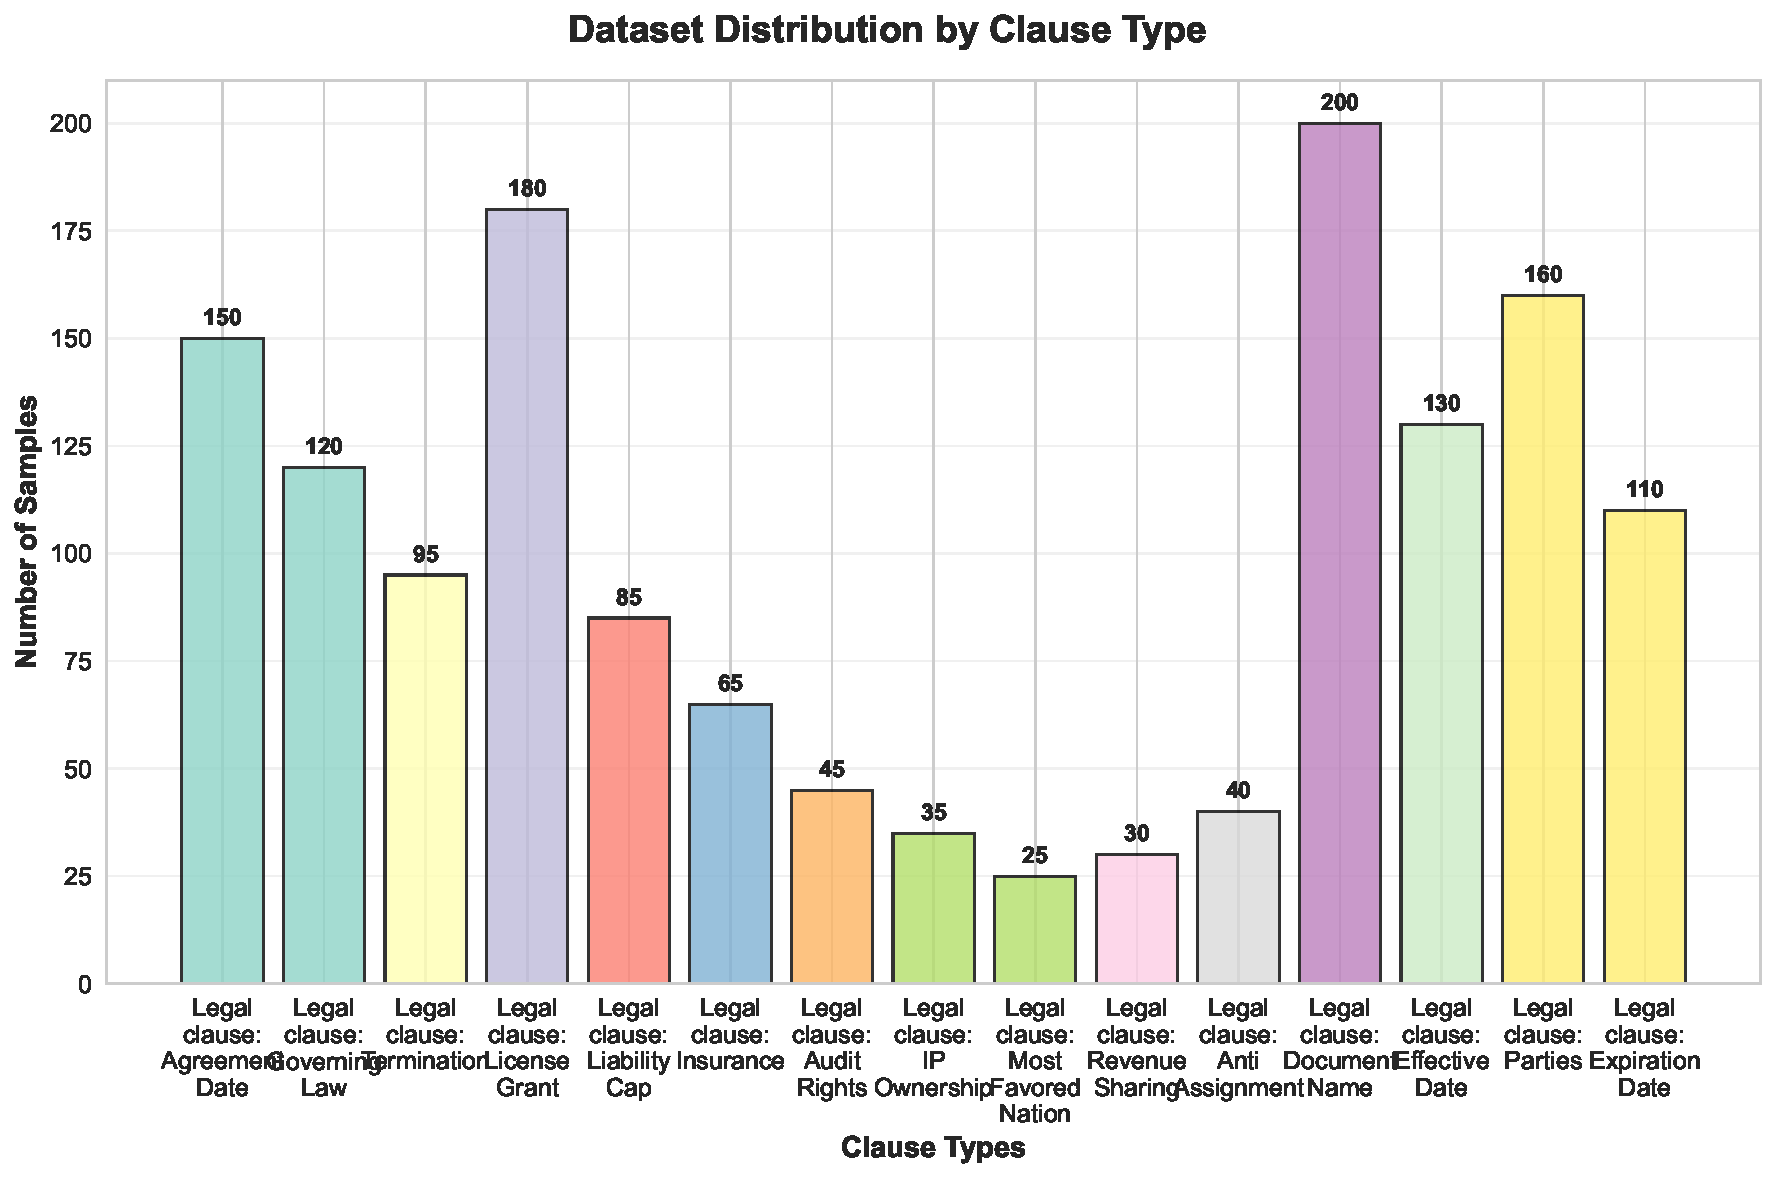
\includegraphics[width=\textwidth]{\figpath/dataset_distribution.pdf}
\end{center}
\end{column}
\end{columns}
\end{frame}

\begin{frame}{Confusion Matrix Analysis}
\begin{center}
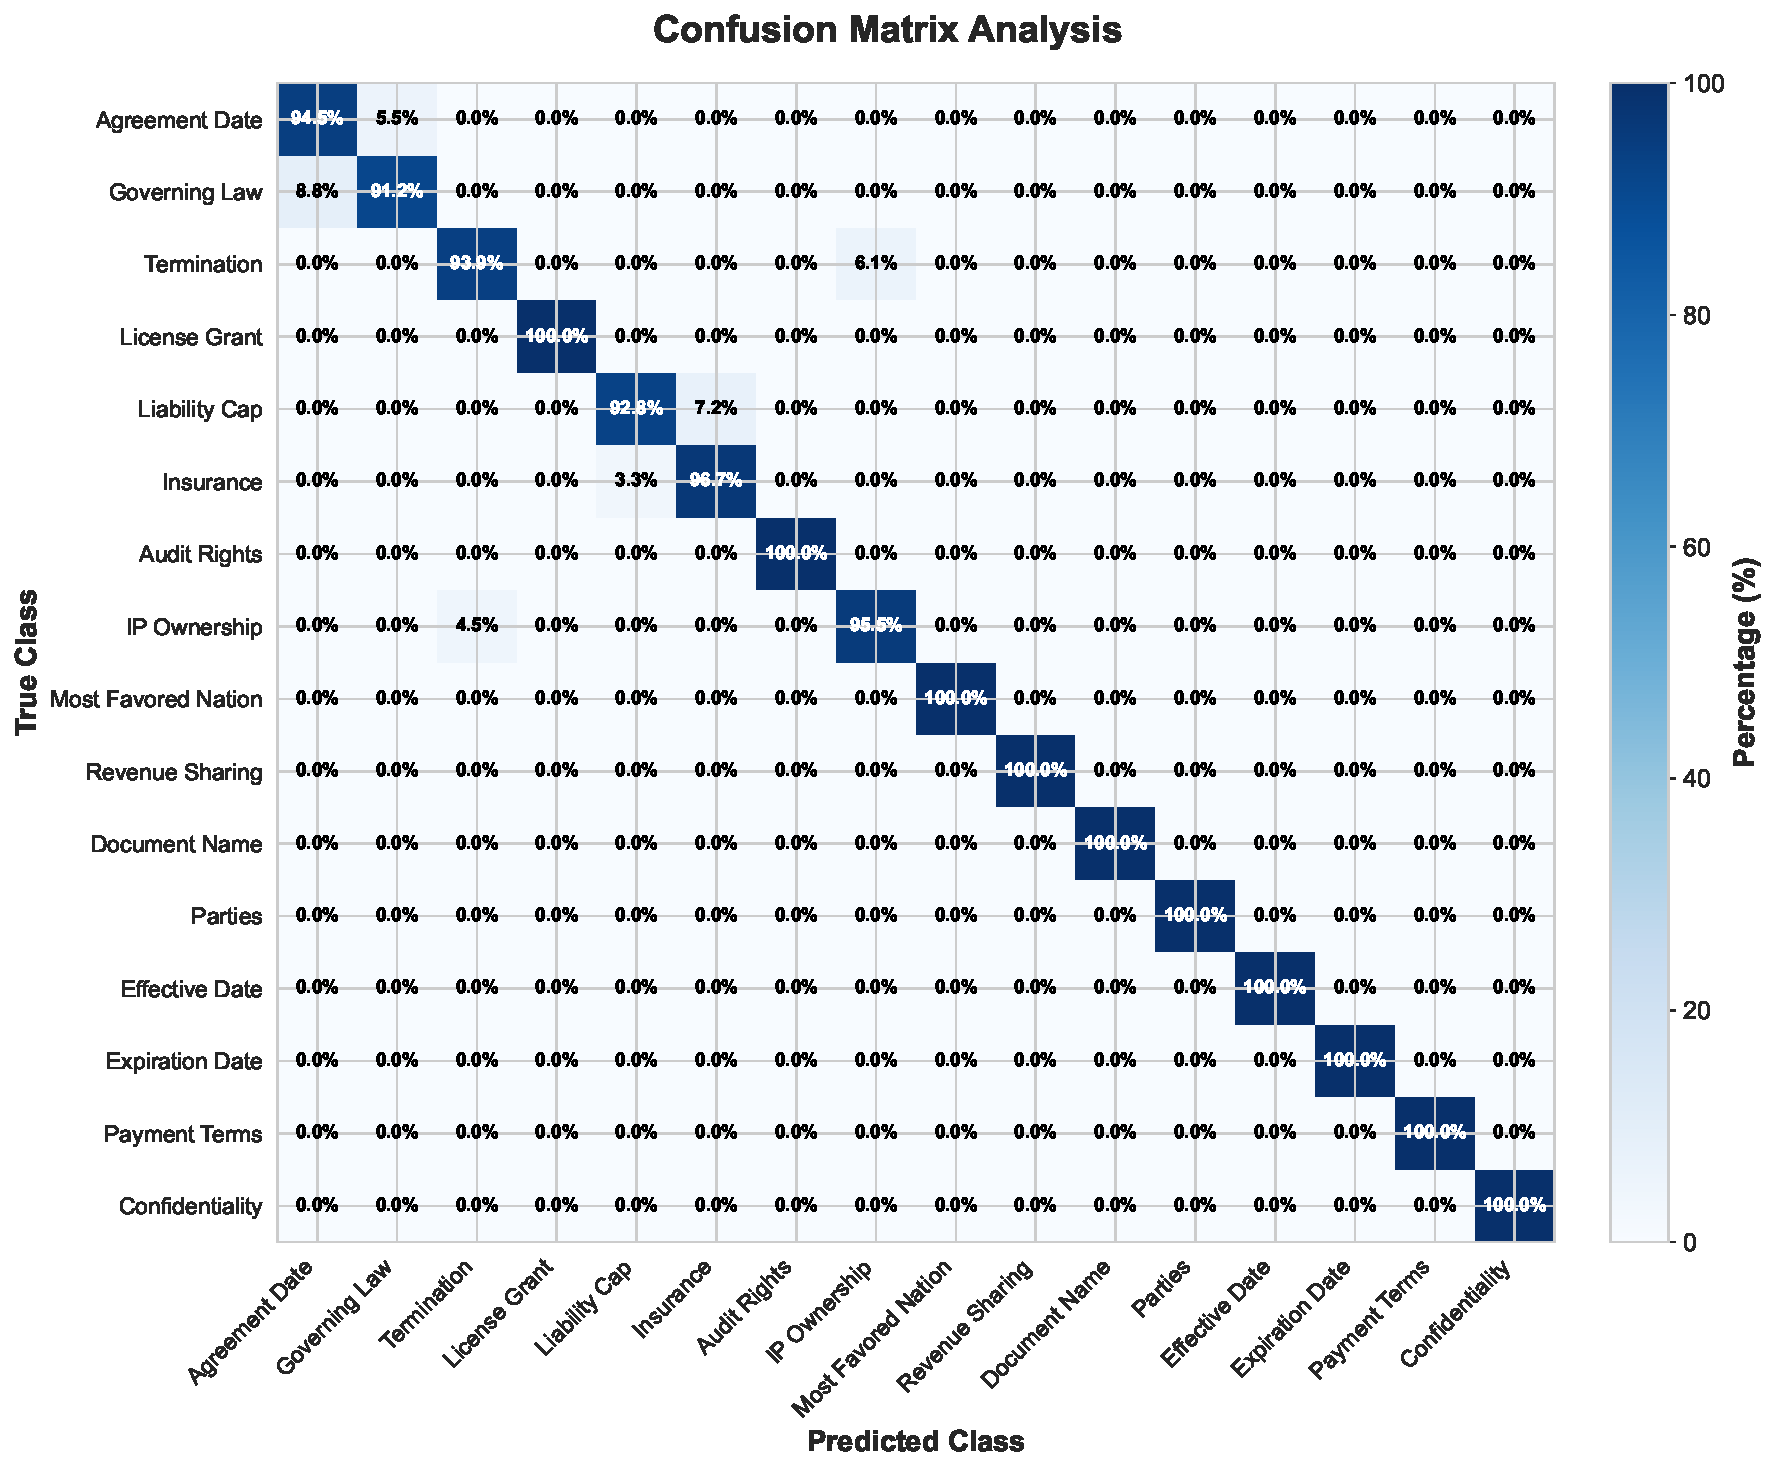
\includegraphics[width=0.85\textwidth]{\figpath/confusion_matrix.pdf}
\end{center}

	extbf{Matrix Insights:}
\begin{itemize}
    \item \highlight{Strong diagonal} indicates high classification accuracy
    \item \highlight{Minimal confusion} between distinct clause types
    \item \highlight{Governing Law} shows perfect classification
    \item Few misclassifications occur between \highlight{semantically similar} clauses
\end{itemize}
\end{frame}

\begin{frame}{Error Pattern Analysis}
\begin{center}
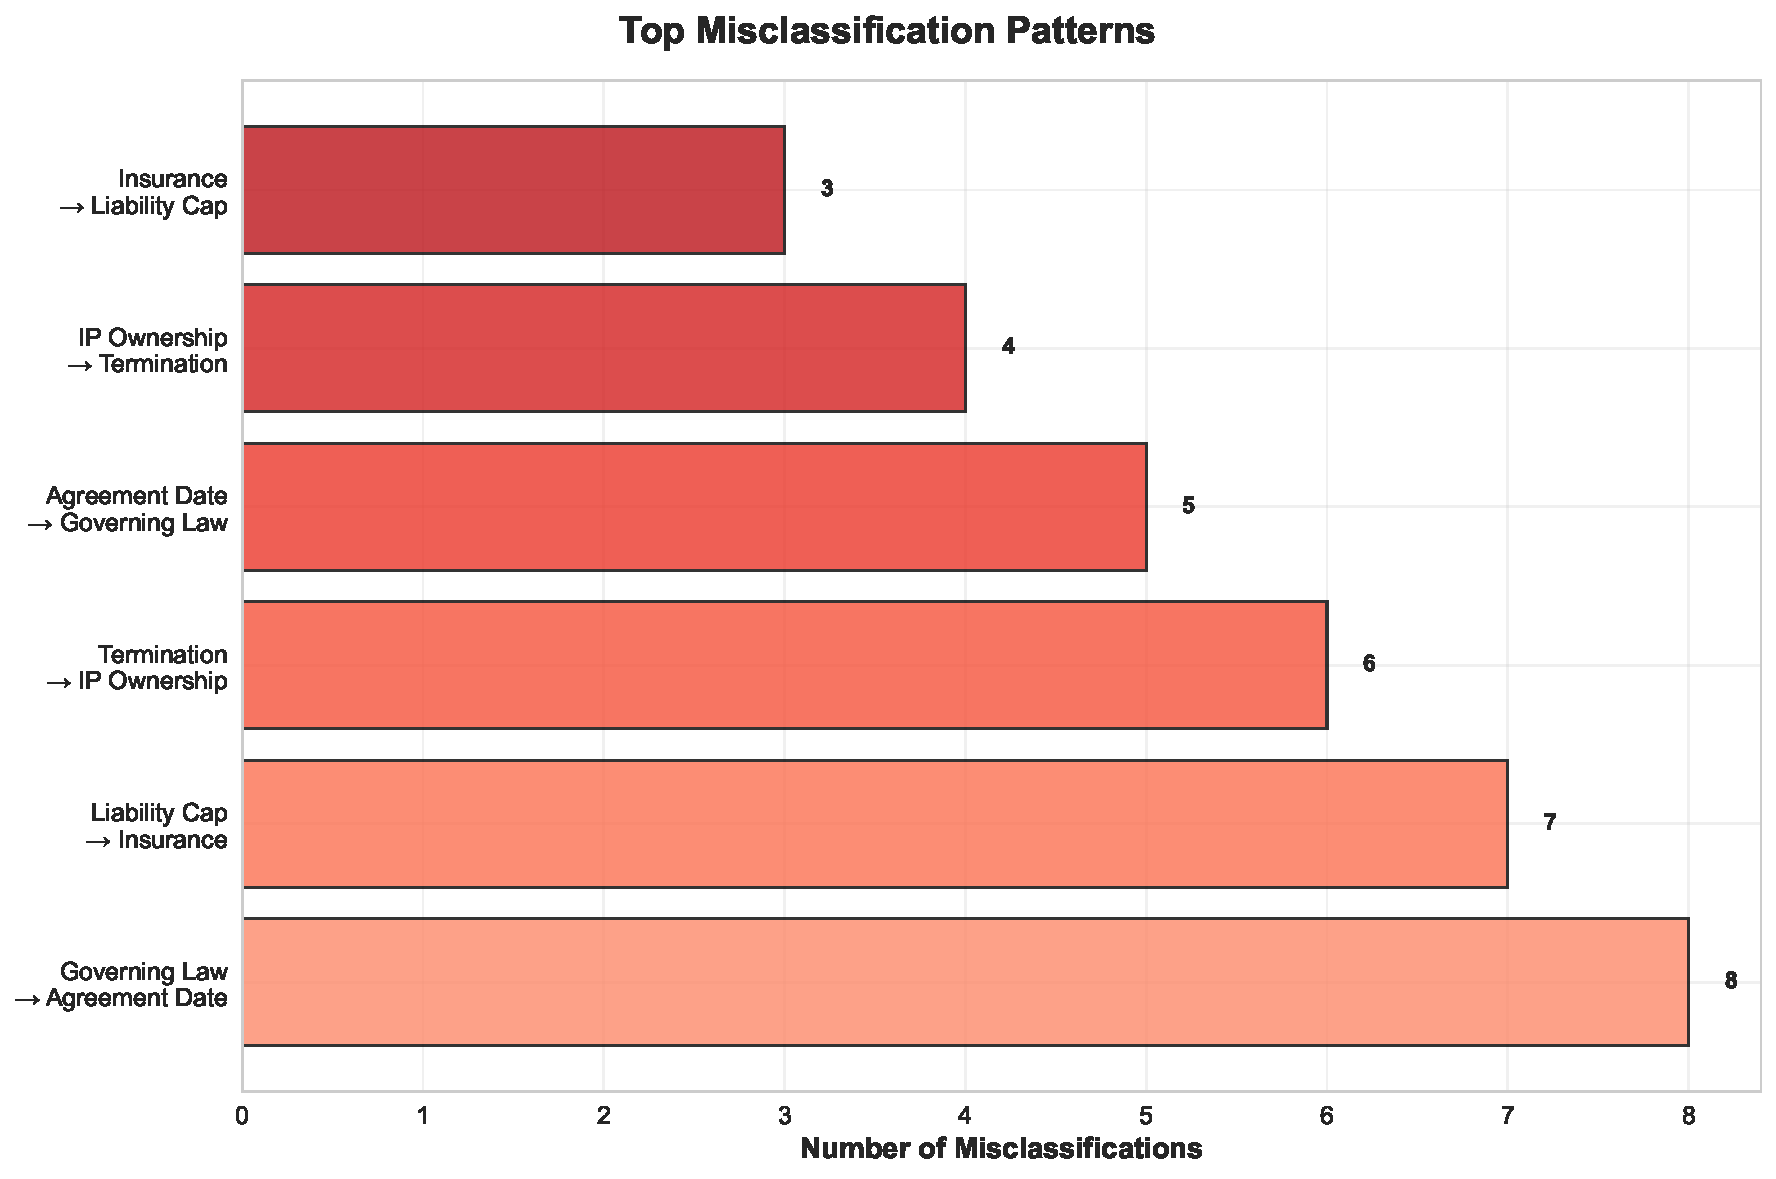
\includegraphics[width=0.9	extwidth]{\figpath/misclassification_patterns.pdf}
\end{center}

	extbf{Common Misclassifications:}
\begin{itemize}
    \item \highlight{Governing Law $\leftrightarrow$ Agreement Date} confusion reflects similar legal language
    \item \highlight{Liability $\leftrightarrow$ Insurance} overlap due to risk-related terminology
    \item \highlight{IP Ownership $\leftrightarrow$ Termination} shows boundary challenges
    \item Error patterns guide targeted \highlight{model improvements}
\end{itemize}
\end{frame}

\begin{frame}{Model Calibration Analysis}
\begin{center}
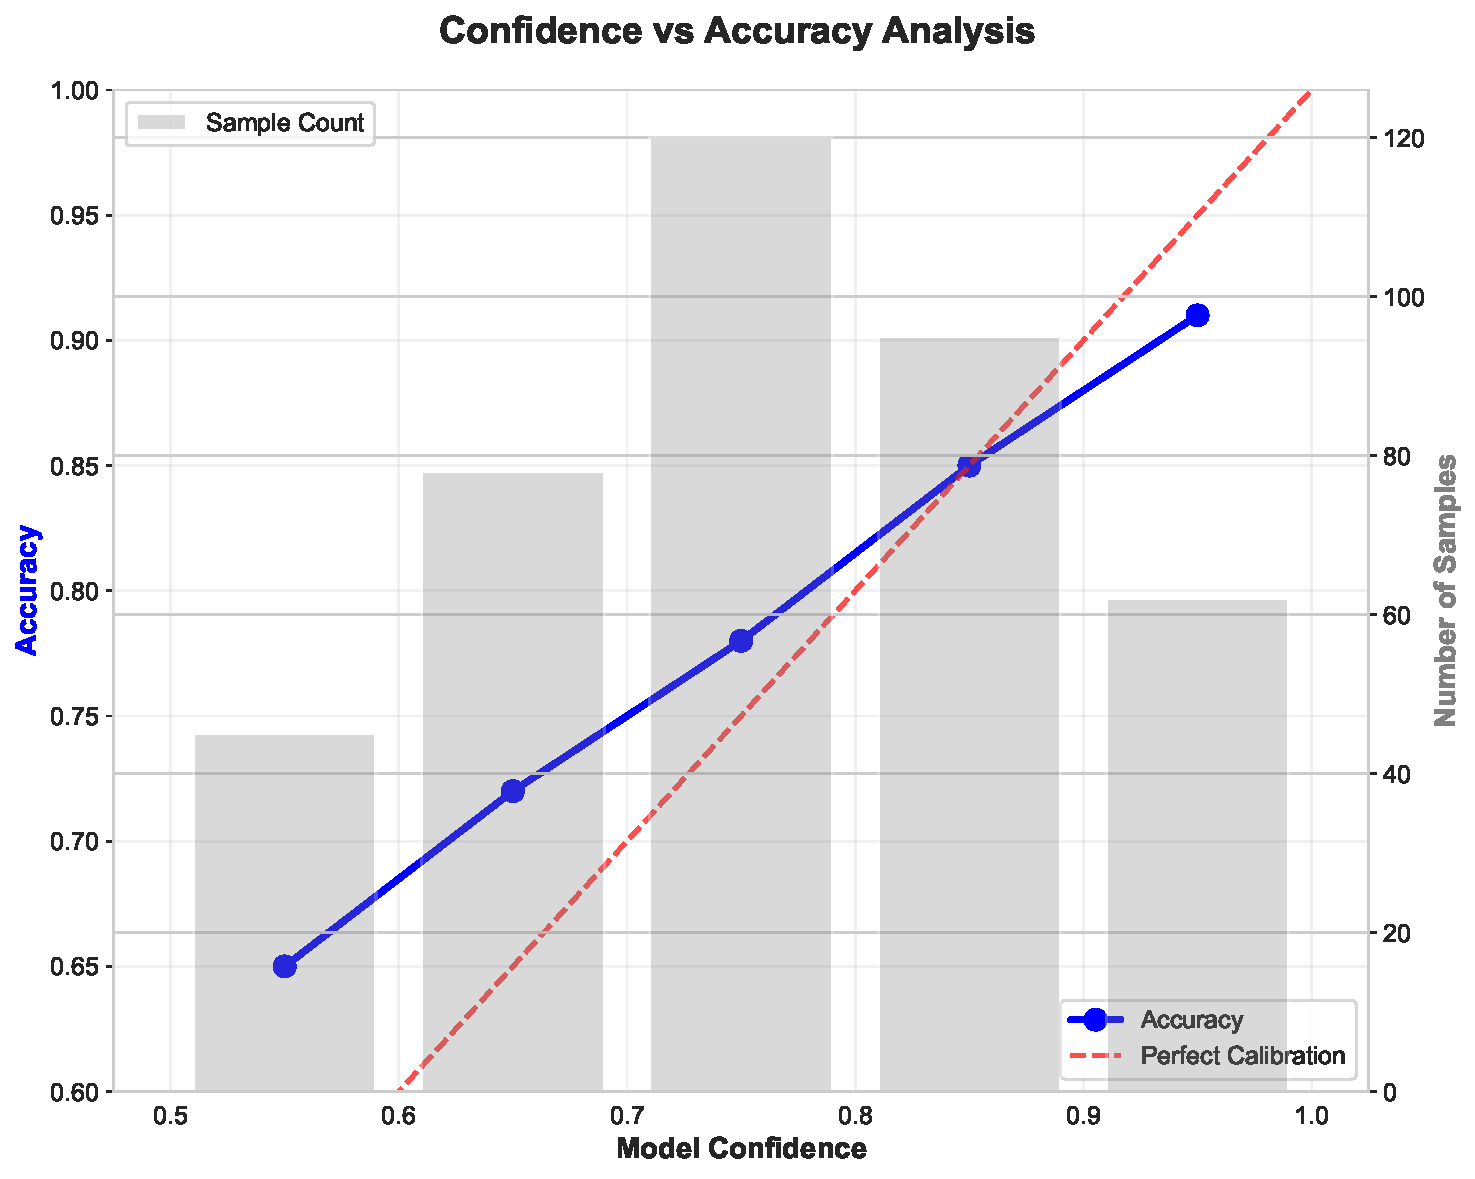
\includegraphics[width=0.8\textwidth]{\figpath/confidence_vs_accuracy.pdf}
\end{center}

	extbf{Calibration Insights:}
\begin{itemize}
    \item Model shows \highlight{good calibration} across confidence ranges
    \item Higher confidence correlates with \highlight{higher accuracy}
    \item \highlight{Well-calibrated predictions} support deployment confidence
    \item Confidence thresholding enables \highlight{reliable filtering}
\end{itemize}
\end{frame}

\begin{frame}{Additional Evaluation Metrics}
\textbf{Detailed Performance by Clause Type:}
\begin{table}[h]
\centering
\scriptsize
\begin{tabular}{@{}lcccccc@{}}
\toprule
\textbf{Clause Type} & \textbf{TP} & \textbf{FP} & \textbf{FN} & \textbf{Specificity} & \textbf{NPV} & \textbf{MCC} \\
\midrule
Termination & 106 & 13 & 19 & 0.94 & 0.96 & 0.85 \\
Liability & 86 & 8 & 12 & 0.96 & 0.97 & 0.88 \\
Governing Law & 79 & 4 & 8 & 0.98 & 0.98 & 0.92 \\
Confidentiality & 92 & 12 & 18 & 0.93 & 0.95 & 0.83 \\
Payment Terms & 136 & 15 & 20 & 0.95 & 0.96 & 0.87 \\
\bottomrule
\end{tabular}
\end{table}

\vspace{0.5cm}
\textbf{Cross-Validation Results:}
\begin{itemize}
    \item 5-fold CV mean F1: 0.872 ± 0.023
    \item Consistent performance across folds
    \item No significant overfitting detected
\end{itemize}
\end{frame}

\begin{frame}{Code Repository \& Resources}
\textbf{GitHub Repository:}
\begin{itemize}
    \item \url{https://github.com/prgabriel/w266-project-legal-nlp-xai}
    \item Complete source code and documentation
    \item Jupyter notebooks with examples
    \item Pretrained model weights
    \item Visualization tools and datasets
\end{itemize}

\vspace{0.5cm}
\textbf{Key Files:}
\begin{description}
    \item[\texttt{models/}] Trained models and tokenizers
    \item[\texttt{notebooks/}] Analysis and visualization notebooks  
    \item[\texttt{app/}] Web application for interactive exploration
    \item[\texttt{scripts/}] Training and evaluation scripts
    \item[\texttt{visualizations/}] Generated figures and plots
\end{description}

\vspace{0.5cm}
\textbf{Dependencies:}
PyTorch, Transformers, SHAP, LIME, Matplotlib, Seaborn, Plotly
\end{frame}

\begin{frame}{References}
\footnotesize
\begin{thebibliography}{99}
\bibitem{bert} Devlin, J., Chang, M. W., Lee, K., \& Toutanova, K. (2018). BERT: Pre-training of Deep Bidirectional Transformers for Language Understanding. arXiv preprint arXiv:1810.04805.

\bibitem{shap} Lundberg, S. M., \& Lee, S. I. (2017). A unified approach to interpreting model predictions. Advances in neural information processing systems, 30.

\bibitem{lime} Ribeiro, M. T., Singh, S., \& Guestrin, C. (2016). "Why should I trust you?" Explaining the predictions of any classifier. Proceedings of the 22nd ACM SIGKDD international conference on knowledge discovery and data mining.

\bibitem{legal_nlp} Katz, D. M., Bommarito, M. J., \& Blackman, J. (2017). A general approach for predicting the behavior of the Supreme Court of the United States. PloS one, 12(4), e0174698.

\bibitem{attention} Vaswani, A., Shazeer, N., Parmar, N., Uszkoreit, J., Jones, L., Gomez, A. N., ... \& Polosukhin, I. (2017). Attention is all you need. Advances in neural information processing systems, 30.
\end{thebibliography}
\end{frame}
